% Opcje klasy 'iithesis' opisane sa w komentarzach w pliku klasy. Za ich pomoca
% ustawia sie przede wszystkim jezyk oraz rodzaj (lic/inz/mgr) pracy.
\documentclass[shortabstract, english, inz]{iithesis}

\usepackage[utf8]{inputenc}

%%%%% DANE DO STRONY TYTUŁOWEJ
% Niezaleznie od jezyka pracy wybranego w opcjach klasy, tytul i streszczenie
% pracy nalezy podac zarowno w jezyku polskim, jak i angielskim.
% Pamietaj o madrym (zgodnym z logicznym rozbiorem zdania oraz estetyka) recznym
% zlamaniu wierszy w temacie pracy, zwlaszcza tego w jezyku pracy. Uzyj do tego
% polecenia \fmlinebreak.
\polishtitle    {Porównanie wydajności \fmlinebreak różnych implementacji algorytmu Wave Function Collapse}
\englishtitle   {Performance comparison of Wave Function Collapse Algorithm implementations}
\polishabstract {Algorytm Wave Function Collapse (WFC) autorstwa Maxim'a Gumin'a służy do proceduralnego tworzenia treści (ang. procedural content generation PCG) w oparciu o przykładowe obrazy i jest przykładem algorytmu probabilistycznego. Dla uzyskania podobieństwa pomiędzy danymi wejściowymi a wynikiem, algorytm składa obraz z fragmentów wejścia przestrzegając zasad sąsiedztwa z oryginalnego obrazu. Ten dokument opisuje zasady działania WFC, jego zastosowania i analizę wydajności różnych implementacji wariantu algorytmu służącego do tworzenia trójwymiarowego modelu w oparciu o zestaw klocków (ang. tileset) w tym moje autorskie pomysły na poprawę wydajności tego algorytmu.\fmlinebreak\url{https://github.com/KrzysiekSlawik/wfc}}
\englishabstract{Wave Function Collapse (WFC) algorithm by Maxim Gumin can be used for procedural content generation (PCG) and is an example of an probabilistic algorithm. It's input is example image and it's output is image following input style by using parts of example image and respecting neighbor relation between them. This paper aims at describing theory behind WFC, where it can be applied and performance comparison of implementations of WFC variant that serves as tilemap generator including my original ideas for performance improvement of the algorithm. \fmlinebreak\url{https://github.com/KrzysiekSlawik/wfc}}
% w pracach wielu autorow nazwiska mozna oddzielic poleceniem \and
\author         {Krzysztof Sławik}
% w przypadku kilku promotorow, lub koniecznosci podania ich afiliacji, linie
% w ponizszym poleceniu mozna zlamac poleceniem \fmlinebreak
\advisor        {dr Łukasz Piwowar}
\date          {03.02.2023}                     % Data zlozenia pracy
% Dane do oswiadczenia o autorskim wykonaniu
\transcriptnum {307020}                     % Numer indeksu
\advisorgen    {dr. Łukasza Piwowara} % Nazwisko promotora w dopelniaczu
%%%%%

%%%%% WLASNE DODATKOWE PAKIETY
%
%\usepackage{graphicx,listings,amsmath,amssymb,amsthm,amsfonts,tikz}
%
\usepackage{url}
\usepackage{graphicx}
\usepackage{float}
\usepackage{subcaption}
\usepackage[sorting=none]{biblatex}
\addbibresource{bibliography.bib}
%%%%% WŁASNE DEFINICJE I POLECENIA
%
%\theoremstyle{definition} \newtheorem{definition}{Definition}[chapter]
%\theoremstyle{remark} \newtheorem{remark}[definition]{Observation}
%\theoremstyle{plain} \newtheorem{theorem}[definition]{Theorem}
%\theoremstyle{plain} \newtheorem{lemma}[definition]{Lemma}
%\renewcommand \qedsymbol {\ensuremath{\square}}
% ...
%%%%%

\begin{document}

%%%%% POCZĄTEK ZASADNICZEGO TEKSTU PRACY

\chapter{Introduction}
This chapter briefly describes WFC, its background, roots and use cases.
\section{Texture Synthesis}
\begin{figure}[H]
\centering
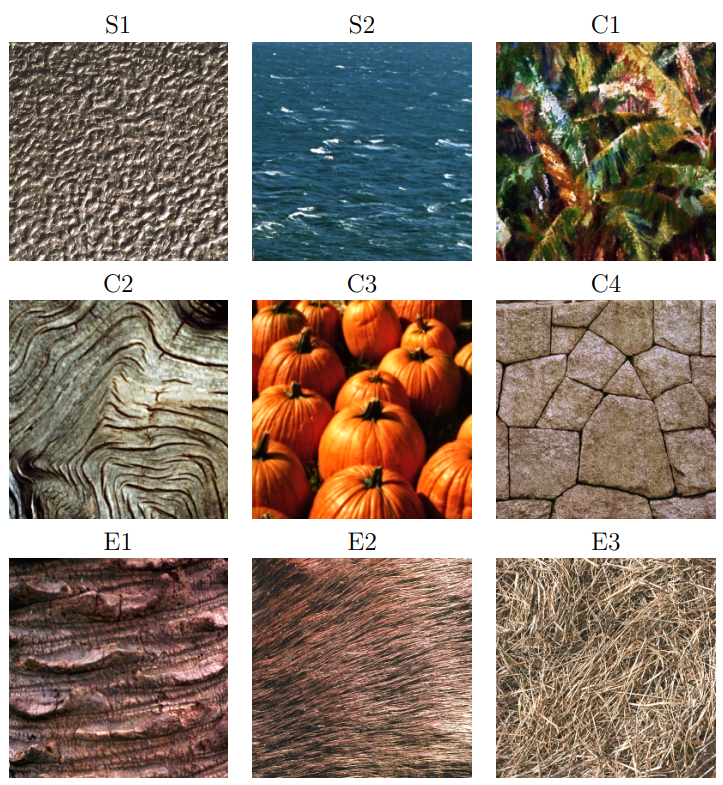
\includegraphics[width=0.75\textwidth, angle=0]{images/texsynth_input.png}
\caption{Input images for Patchwork texture synthesis (Source: \cite{harrison2002patchwork})}
\label{fig:texSynthIn}
\end{figure}
\begin{figure}[H]
\centering
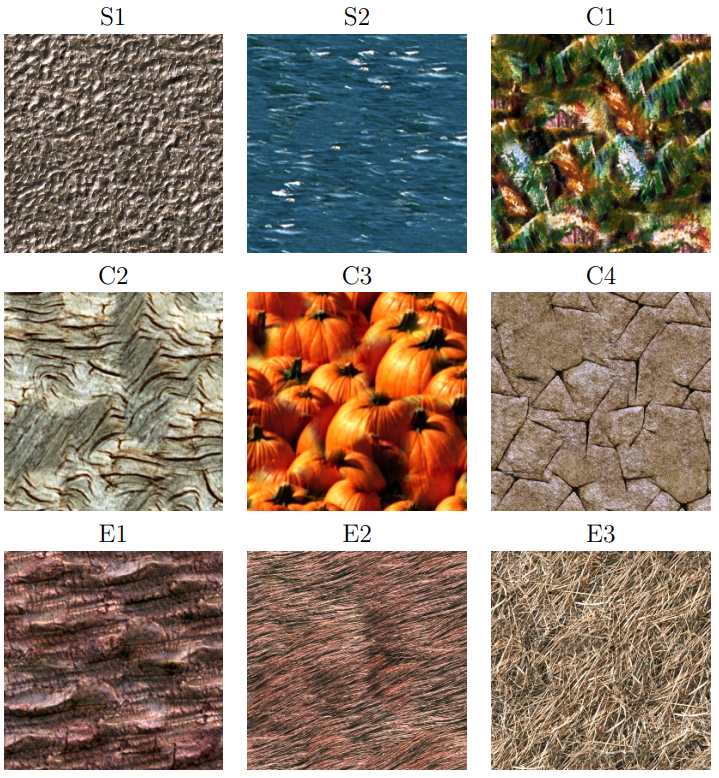
\includegraphics[width=0.75\textwidth, angle=0]{images/texsynth_output.png}
\caption{Output images for Patchwork texture synthesis (Source: \cite{harrison2002patchwork})}
\label{fig:texSynthOut}
\end{figure}
In computer graphics, texture synthesis is the problem of generating the output image that is bigger than the input image whilst resembling it. Most of techniques solving this problem aim at having high similarity of patterns which are sub-images of small sizes (e.g. 5x5 pixels). It is worth to mention that similarity, in most of the cases, is based on Euclidean distance of pixel colours, whereas in case of WFC patterns have to be exact match.\cite{Smith}
Requirement of exact match of patterns allowes for much wider use of WFC than other typical texture synthesis tools as with little adjustments user can easily define key features of the output image. \cite{GraphBased}
\begin{figure}[H]
\centering
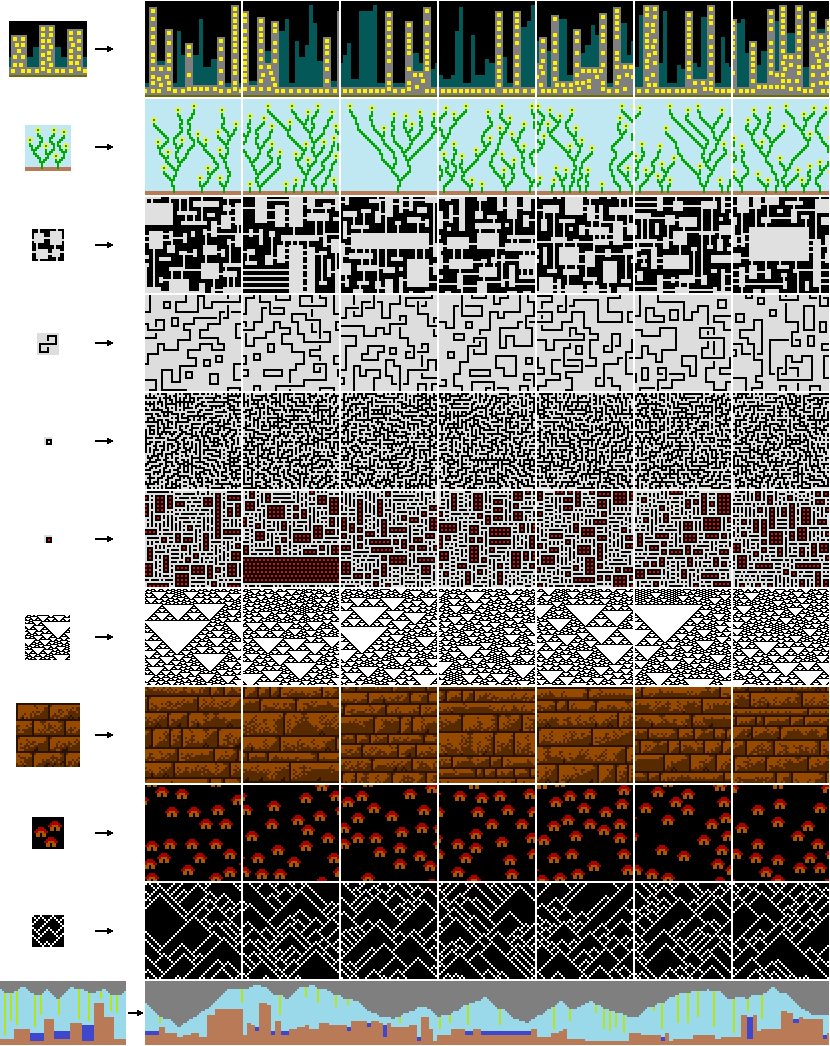
\includegraphics[width=0.75\textwidth, angle=0]{images/wfc.png}
\caption{Examples of inputs and outputs of the WFC algorithm (Source: \cite{MaximGumin})}
\label{fig:wfc}
\end{figure}
As stated by Maxim Gumin, WFC tends to be slower than P. F. Harrison's texture synthesis  algorithm (examples see \ref{fig:texSynthIn} \ref{fig:texSynthOut}) but strict relation in which patterns have to be in images produced by WFC allowes for capturing long correlations like pattern of bricks, greenery or abstract shapes with a pixel perfect precision, which makes it perfect candidate to use with pixel art and for level generation. See \ref{fig:wfc}.\cite{MaximGumin}


\section{Constraint Solving Algorithms}
\begin{figure}[H]
\centering
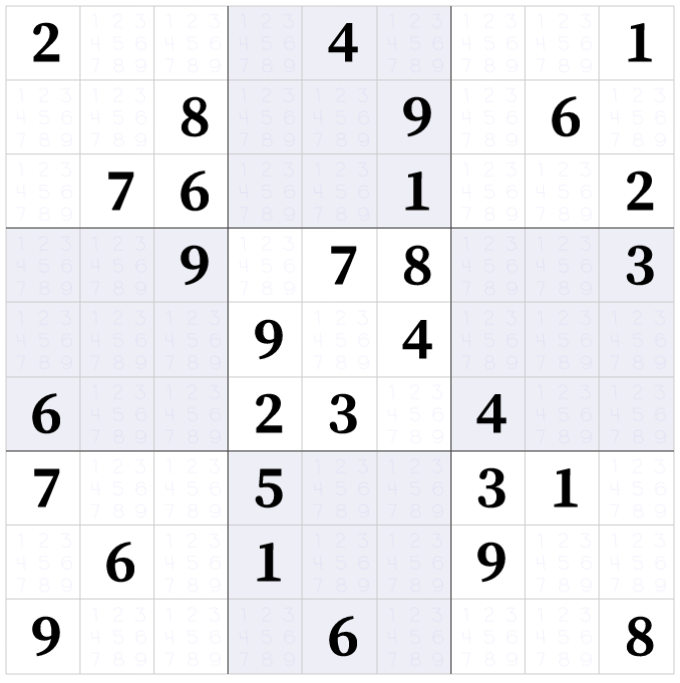
\includegraphics[width=0.75\textwidth, angle=0]{images/sudoku.png}
\caption{Example Sudoku problem (Source: \cite{sudoku})}
\label{fig:sudoku}
\end{figure}
Constraint satisfaction problems (CSPs) are typically defined in terms of decision variables and values. An example of CSP might be the Sudoku game (\ref{fig:sudoku}) in which each location on the grid is variable and values come from digits set. The goal of an algorithm solving CSPs is to find a total assignment (each variable has assigned value) that does not violate any constraints. \fmlinebreak
WFC algorithm constructs solution image by assigning values from discrete set of unique local patterns from input image. \cite{Smith} The key observation is that WFC being CSP solver means that each iteration (every step of algorithm assigning to variable) produces new valid CSP. This can be used to guide WFC by assigning some variables by hand, as partially solved CSP is still proper input for any CSP solver. (as long as partial assignment does not violate constraints)
\section{Procedural Content Generation}
PCG is powerful tool wherever high or endless amount of content is required as PCG can reduce the resources spent on new assets by generating them based on those already manually created by artists or creating them entirely basing on rules predefined in algorithm. An important factor is making decision on when to use PCG is cost of preparation algorithm compared with cost of manually making all assets. In case of products that require endless amount of assets PCG is only available option and it has to be highly controlled process. The upfront cost of using PCG comes from choosing well fitted method, parameter tuning, deeply understanding design and knowing how to encode it.
From game development point of view two types of PCG can be distinguished. Offline PCG is used for creating assets during development, it doesn't have to produce output in real time and its output can be checked by artists before being used in final product. On the other hand online PCG is used in final application runtime. It has to work in real time and produce its output in acceptable loading screen time. Artists can't check algorithm outputs so it has to be highly controllable and fine tuned during development phase.\cite{DesignLevelConstraints}\break\break
WFC algorithm main advantages in PCG are ease of use as basic results can be achieved by tuning input image only, high controllability as strict neighbor relations can guarantee generation of playable content, easily extended as adding additional rules like density, total count, distance on top of neighbor relations. \cite{Smith, DesignLevelConstraints}

\section{Chapters Summary}
Short summary of the following chapters:
\begin{itemize}
    \item \ref{chapter2}. WFC Applications - notable examples of how WFC might be used
    \item \ref{chapter3}. The WFC Algorithm - description and analysis of the original algorithm
    \item \ref{chapter4}. Performance Comparison - analysis of performance of WFC algorithm implemented by me, comparison of different used improvements
    \item \ref{chapter5}. Technical - how to install and test my code, technologies used
    \item \ref{chapter6}. Summary And Future Work - short description of obtained results and ideas for future development.
\end{itemize}



\chapter{WFC Applications}
\label{chapter2}
\section{level generation}
\begin{figure}[H]
\centering
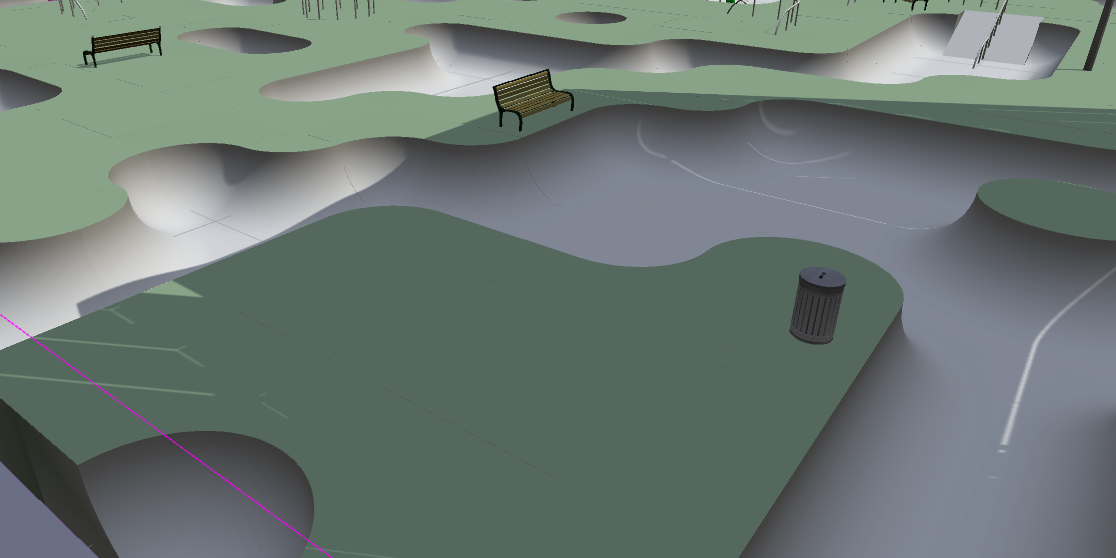
\includegraphics[width=0.75\textwidth, angle=0]{images/skater.png}
\caption{Proc Skater - first game in which WFC was used for level generation (Source: \cite{skater})}
\label{fig:skater}
\end{figure}
WFC algorithm appeared in a game for the first time during the ProcJam event in form of a submission from Joseph Parker, Ryan Johns and Oscar Morante - Proc Skater game \ref{fig:skater}. As stated by Joseph Parker, he has “never been this excited about an algorithm!”. In case of their game use of WFC ensured smooth traversability of the level thanks to exact pattern matching used by the algorithm.\break
 Oskar Stålberg is another game developer that participated in popularization of WFC algorithm by creating small demo web application\footnote{Demo of WFC by  Oskar Stålberg \url{http://oskarstalberg.com/game/wave/wave.html}}. He was one of the first to generalise WFC for other shapes and 3D meshes\footnote{WFC algorithm filling sphere surface with triangle shaped tiles by Oskar Stålberg \url{https://twitter.com/OskSta/status/784847588893814785}}. Oskar Stålberg also contributed with adding backtracking\ref{backtracking} and bit wise operations\ref{bitwise} as performance improvements.\cite{Smith}


\section{solving CSPs}
\begin{figure}[H]
\centering
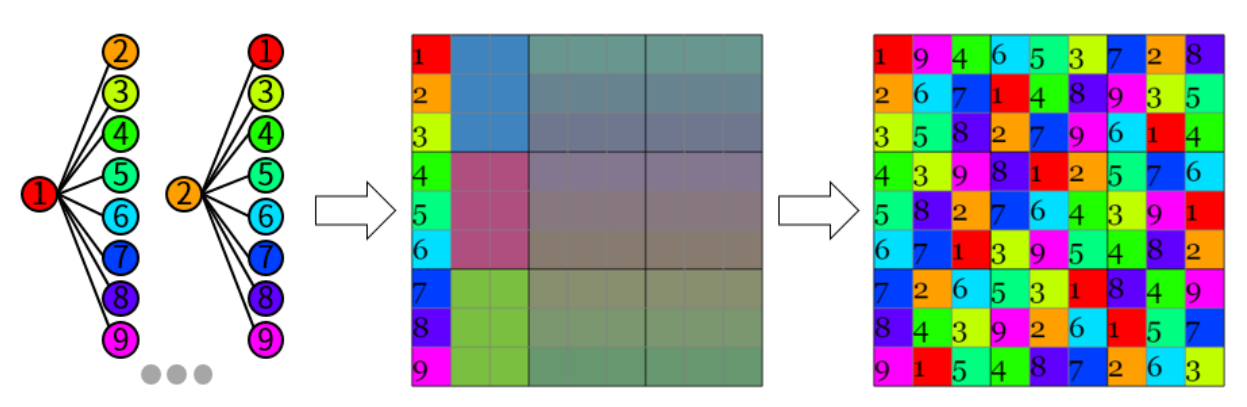
\includegraphics[width=1\textwidth, angle=0]{images/sudoku_solver.png}
\caption{Sudoku allowed neighbors, initial state, puzzle solved using graph based WFC (Source: \cite{GraphBased})}
\label{fig:sudoku_solver}
\end{figure}
WFC algorithm can be used to solve CSPs if properly modified to fit domain. An example would be solving Sudoku game with WFC generalised for graphs which was done as a part of "Automatic Generation of Game Content using a Graph-based Wave Function Collapse Algorithm" \cite{GraphBased}. This paper focused on generalising WFC by allowing each element to have variable amount of neighbors but with a drawback of not distinguishing directions. \footnote{original WFC uses neighbor relations like "A is left neighbor of B" whereas in case of graph based solution we only know that "A is neighbor of B"} For solving the Sudoku game rules can be formulated in a way that fits this model - each variable has 20 neighbors.\ref{fig:sudoku_neighbors}.
\begin{figure}[H]
\centering
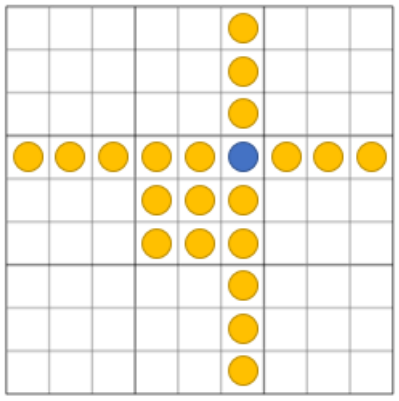
\includegraphics[width=0.50\textwidth, angle=0]{images/sudoku_neighbors.png}
\caption{blue represents selected Sudoku grid element, yellow represents its neighbors (Source: \cite{GraphBased})}
\label{fig:sudoku_neighbors}
\end{figure}
Backtracking \ref{backtracking}had to be added to WFC for it to be able to produce solutions for Sudoku puzzles as contradictions were common due to very strict rules. Even with backtracking WFC is not performing well as a CSP solver, but on the other hand it is able to deduce rules of the problem on its own.\cite{GraphBased}
\begin{figure}[H]
\centering
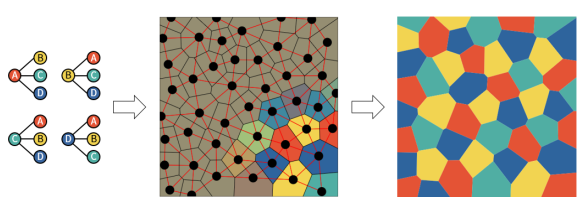
\includegraphics[width=1\textwidth, angle=0]{images/fourcolours.png}
\caption{Four Colours Problem being solved by WFC (Source: \cite{GraphBased})}
\label{fig:fourcolours}
\end{figure}
The same version of WFC was able to solve the four colours problem thanks to it being directly representable as a graph.\ref{fig:fourcolours} Algorithm was able to solve this CSP with basic rules of the four colours problem which it could deduce from example solution, without any additional heuristics.\cite{GraphBased}


\section{writing poetry}
\begin{figure}[H]
\centering
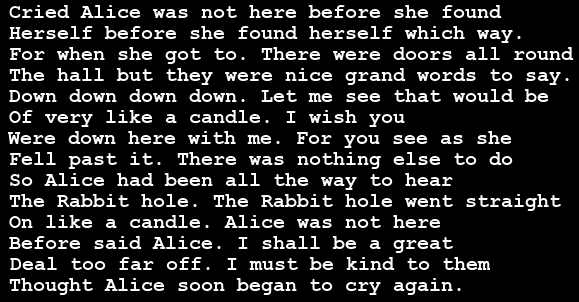
\includegraphics[width=1\textwidth, angle=0]{images/poem.png}
\caption{Poem written by Martin O’Leary WFC inspired algorithm (Source: \cite{wfcpoem})}
\label{fig:poem}
\end{figure}
One of the most unexpected content generated with WFC algorithm is poetry. Martin O’Leary inspired with Maxim Gumin work decided to make WFC that enforced rhyme and meter constraints to generate poetry. Rhyme and meter constraints are long-distance constraints in opposite to originally used neighbor constraints in WFC algorithm. Tiles are created from syllables. Results can be seen at figure \ref{fig:poem}.\cite{Smith, wfcpoem}


\chapter{The WFC Algorithm}
\label{chapter3}
\section{deducing rules}
\section{collapsing states}
\section{propagation of information}
\section{backtracking}
\label{backtracking}
\cite{Smith}



\chapter{Performance Comparison}
\label{chapter4}
    \section{baseline}
        \subsection{code analysis}
        \subsection{performance}
        \subsection{potential improvements}
    \section{Boolean vectors as representation of states \fmlinebreak similar to Maxim Gumin implementation from 2016}
        \subsection{code analysis}
        \subsection{performance}
        \subsection{applied improvements}
    \section{Stack maintaining elements that should be propagated next \fmlinebreak similar to Maxim Gumin current implementation}
        \subsection{pseudo code}
        \subsection{performance}
        \subsection{applied improvements}
    \section{Queue maintaining elements that should be propagated next}
        \subsection{pseudo code}
        \subsection{performance}
        \subsection{comparison with WFC version using stack}
    \section{bit vector as representation for states}
        \label{bitwise}
        \subsection{code analysis}
        \subsection{performance}
        \subsection{potential improvements}
    \section{Fibonacci Heap for faster finding of lowest non-zero entropy}
        \subsection{code analysis}
        \subsection{performance}
        \subsection{potential improvements}
    \section{custom structure for faster finding of lowest non-zero entropy implementing decrease key operation}
        \subsection{comparison with Fibbonacci heap}
    \section{summary}
\chapter{Technical}
\label{chapter5}
    \section{installation instruction}
    \section{technologies used}
\chapter{Summary and Future Work}
\label{chapter6}

%%%%% BIBLIOGRAFIA

%%%%% BIBLIOGRAFIA
\printbibliography[sorting=none]

\end{document}
